\documentclass[aspectratio=169]{beamer}

%%%%%%%%%%%%
%%% PACKAGES
%%%%%%%%%%%%
\usepackage[T1]{fontenc}
\usepackage[sfdefault,scaled=.85]{FiraSans}
\usepackage{newtxsf}
\usepackage{xcolor}
\usepackage{color}
\usepackage{framed}
\usepackage{graphicx}
\usepackage{amsmath}
\usepackage{multicol}
\usepackage{tikz}
\usepackage{siunitx}
\usepackage{pgfplots}
\usepackage[font={footnotesize}]{caption}
\usepackage{setspace}
\usepackage{braket}

%%%%%%%%%%%%%%%%%%
%%% CUSTOMISATIONS
%%%%%%%%%%%%%%%%%%
\usetikzlibrary{intersections}
\pgfplotsset{compat=1.15}
\baselineskip=25pt
\newcommand{\highlight}[1]{\fcolorbox{yellow}{yellow}{#1}}
\usetheme[progressbar=frametitle, numbering=none]{metropolis}
\definecolor{red}{RGB}{150, 20, 20}
\definecolor{grey}{RGB}{150, 150, 150} % 0 (black) to 255 (white)
\definecolor{faded}{RGB}{215, 215, 215}
\definecolor{ash}{RGB}{184, 184, 184}
\setbeamercolor{background canvas}{bg=white}
\setbeamercolor{frametitle}{bg=white, fg=red}
\setbeamercolor{progress bar}{fg=red,bg=faded}

% must add equation numbers in Part 1.
% rewrite sections.
% A better chronological description for blackbody.
% bit of part 2 and 3 are unfinished.
% some statements needs to be rechecked.

\title{Understanding the spectrum of a blackbody}
\institute{\color{grey} Guided by V.H. Belvadi \\ Dept. of Physics \\ Yuvaraja's College, Mysuru}
\author{Sudheendra B.R. \\ Suhas P.K. \\ Shahsank K.K.}
\date{\vspace*{1ex}\color{grey}{\footnotesize March 2020}}

\begin{document}

\begin{frame}[noframenumbering]
	\titlepage
\end{frame}

\section{\textbf{Part 3}}

\begin{frame}{}
\begin{multicols}{3}
 
  \textbf{P} = probability
  
	\columnbreak
	
	$ \phi $ = Probability amplitude

	\columnbreak
	
	\textbf{P} = $ \rvert\,\phi \rvert\,^{2} $
	
	\end{multicols}
	
			 \[ \phi  =  \phi_{1} + \phi_{2} \] 
			 
			 \[ \textbf{P} =  \rvert\,\phi_{1} + \phi_{2} \rvert\,^{2} \]


\end{frame}

\begin{frame}

	\begin{multicols}{2}

		\begin{itemize}
			\item Detector 1 is set to detect only $ \alpha $ particles and Detector 2 is set to detect only oxygen atoms.\pause \newline
			\item Probability amplitude of the scattering is given by $ f(\theta)$ at angle $\theta$.\pause \newline
			\item The probability of this event = $ \,\rvert\,f(\theta) \,\rvert\,^{2} $
		\end{itemize}
		
	\columnbreak

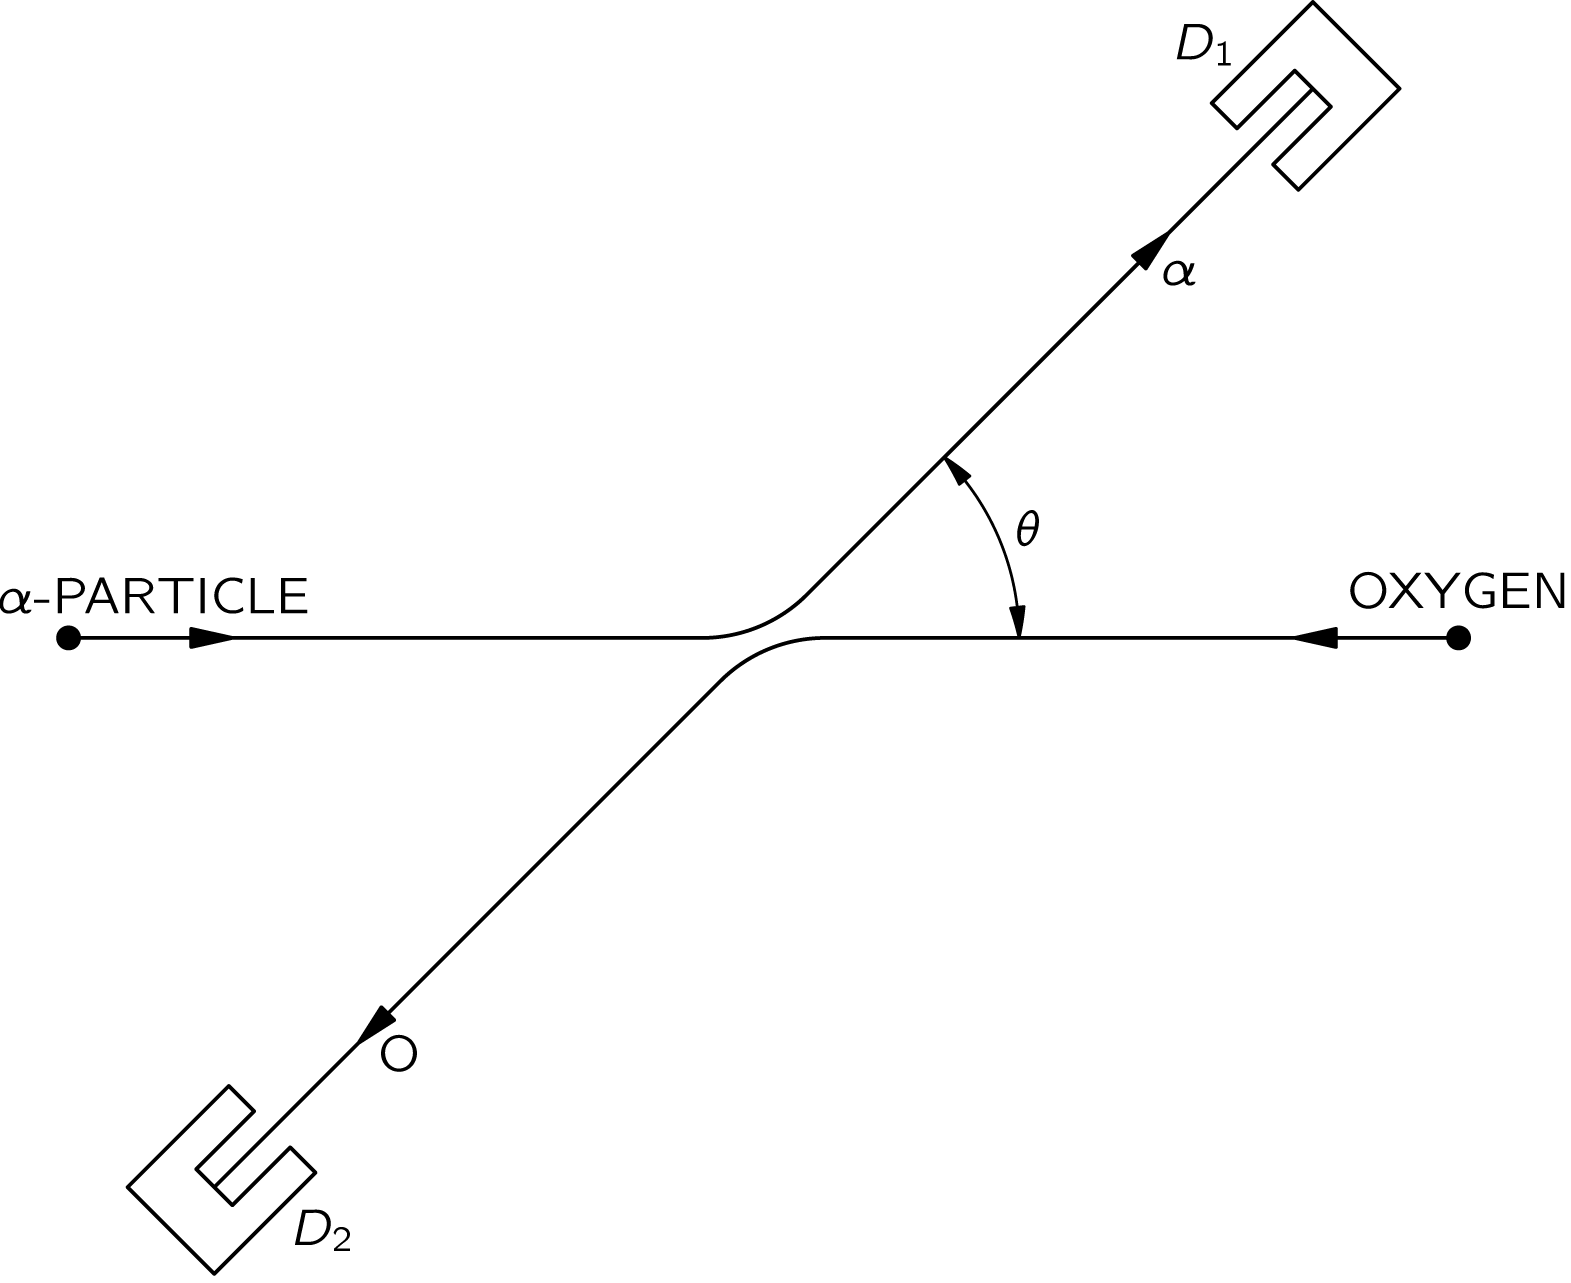
\includegraphics[scale=0.45]{alpha-ox.png}

	\end{multicols}


\end{frame}


\begin{frame}{}

	\begin{multicols}{2}
 
 		\begin{itemize}
	
			\item Set up the detectors such that the detectors would detect either $\alpha$ particle or oxygen atom.\pause \newline
			\item We will not distinguish which particle is which entering the detector.\pause \newline
			\item This means that if oxygen atom in position $\theta$ , then
		$\alpha$ particle on the opposite side is at an angle $\pi-\theta$.
		
		\end{itemize}
	
	\columnbreak
	
		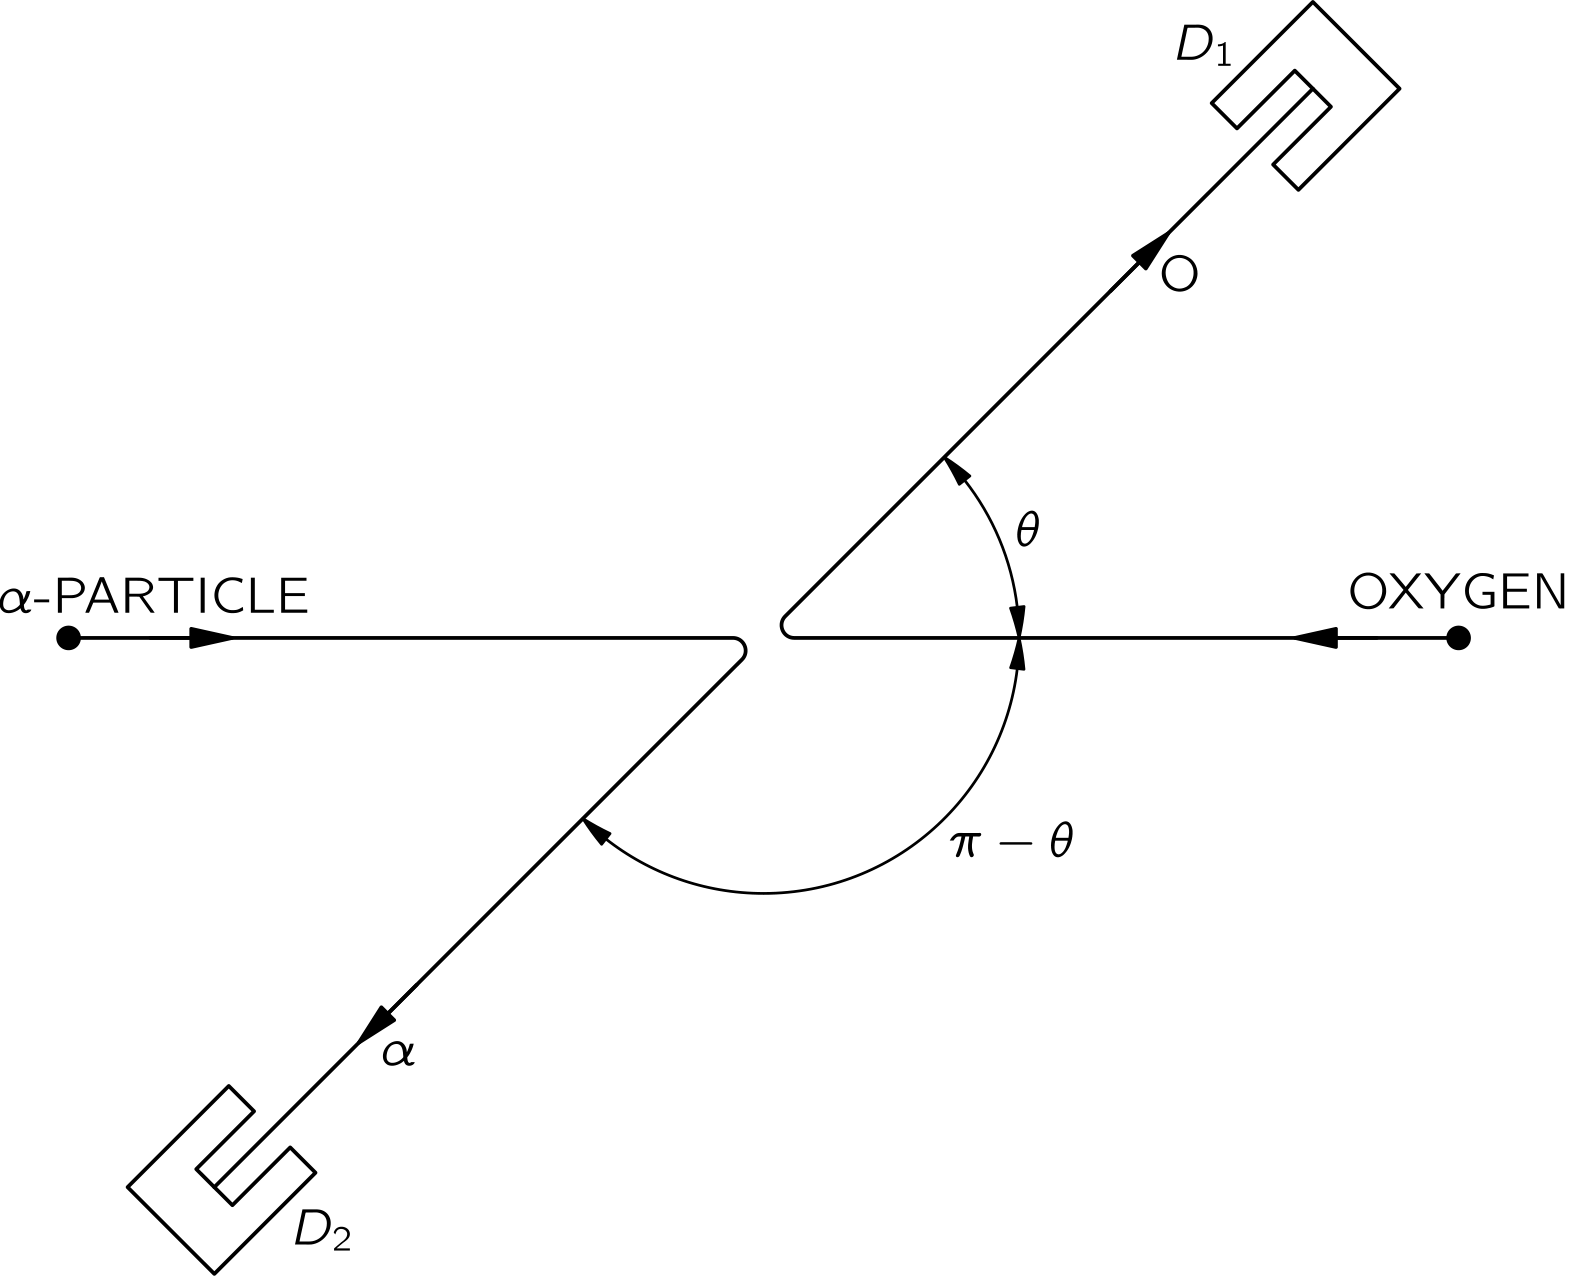
\includegraphics[scale=0.45]{alpha-ox-2.png} 
	
	\end{multicols}
	
		
\end{frame}

\begin{frame}{}


	\begin{multicols}{2}
 
		 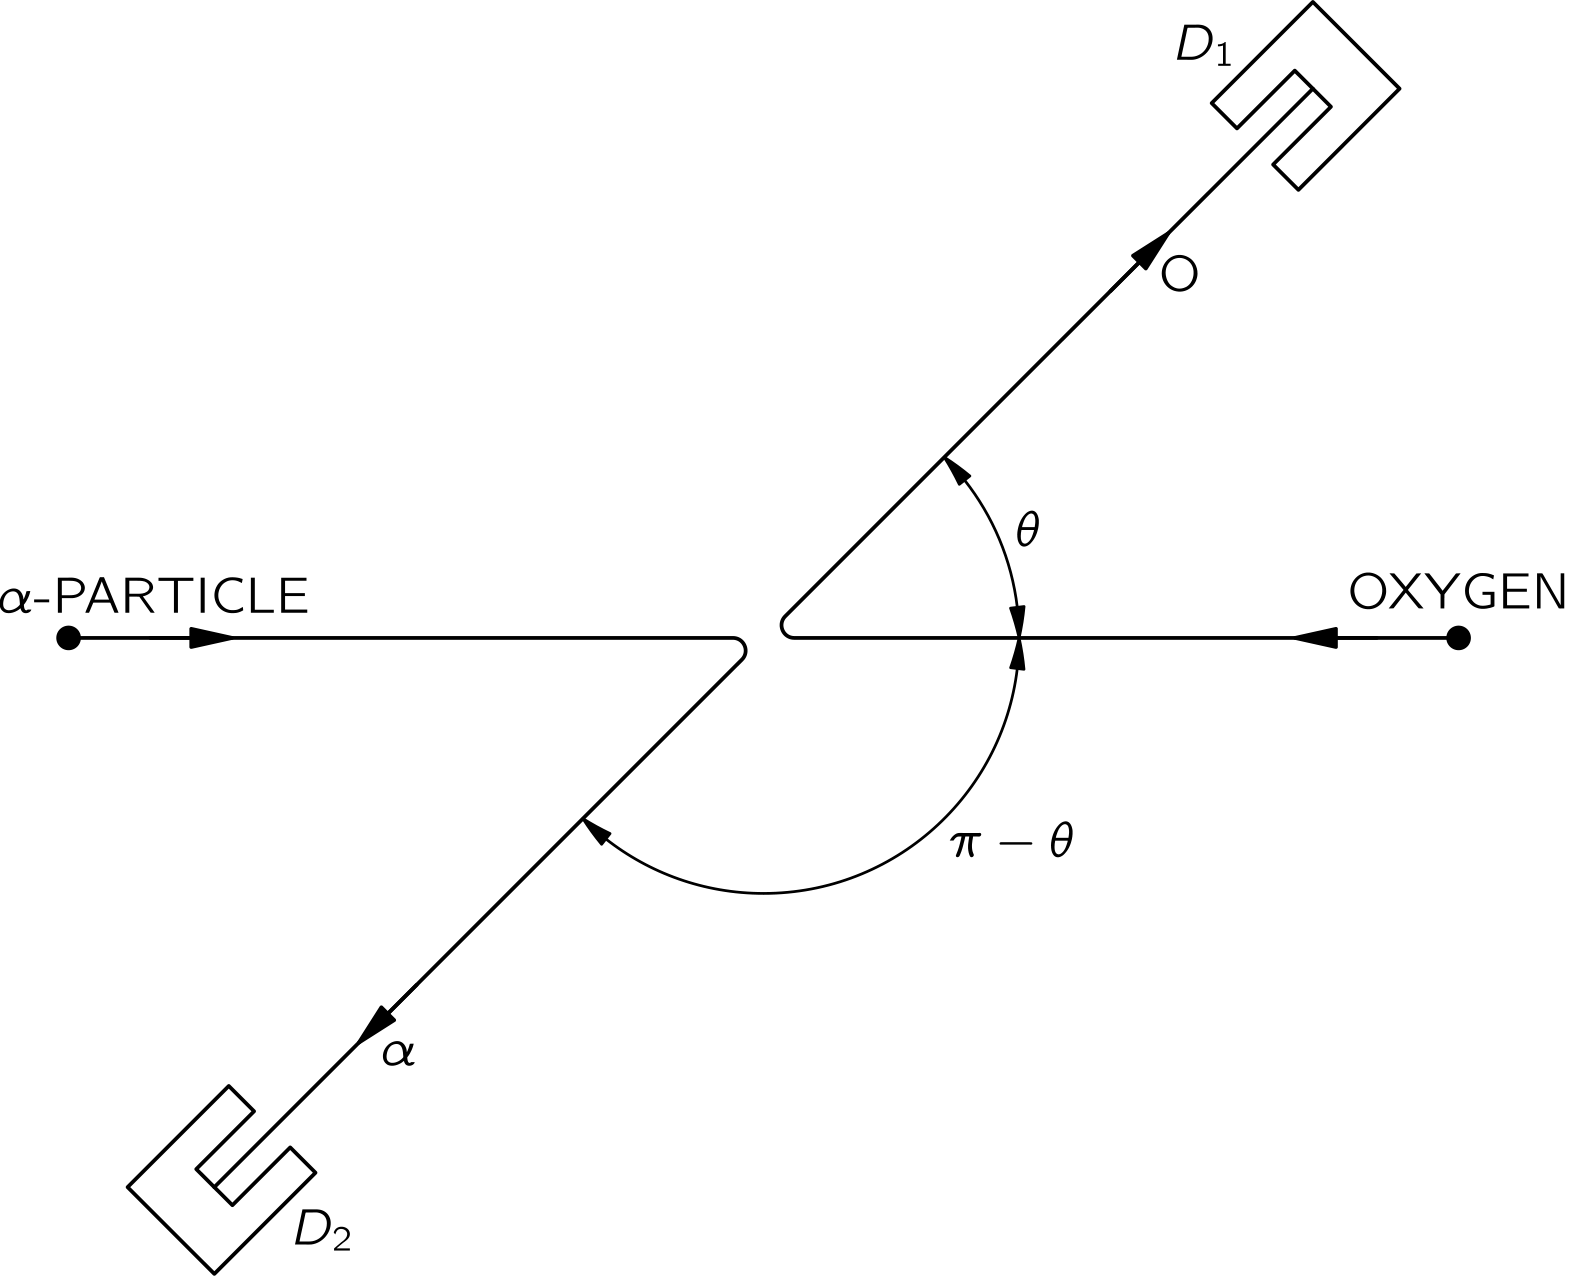
\includegraphics[scale=0.45]{alpha-ox-2.png}
 
	\columnbreak
	
		\begin{itemize}
	
			\item Probability amplitude of oxygen atom = $f(\pi-\theta)$ \pause \newline
			\item Probability amplitude of $\alpha$ particle = $f(\theta)$ \pause \newline
			\item The probability of a particle being detected at detector 1 = $ \rvert\,f(\theta) \rvert\,^{2} $ + $ \rvert\,f(\pi - \theta) \rvert\,^{2} $
		
 		\end{itemize}
 	
	\end{multicols}
	
	
\end{frame}

\begin{frame}

	\begin{multicols}{2}
	
 		 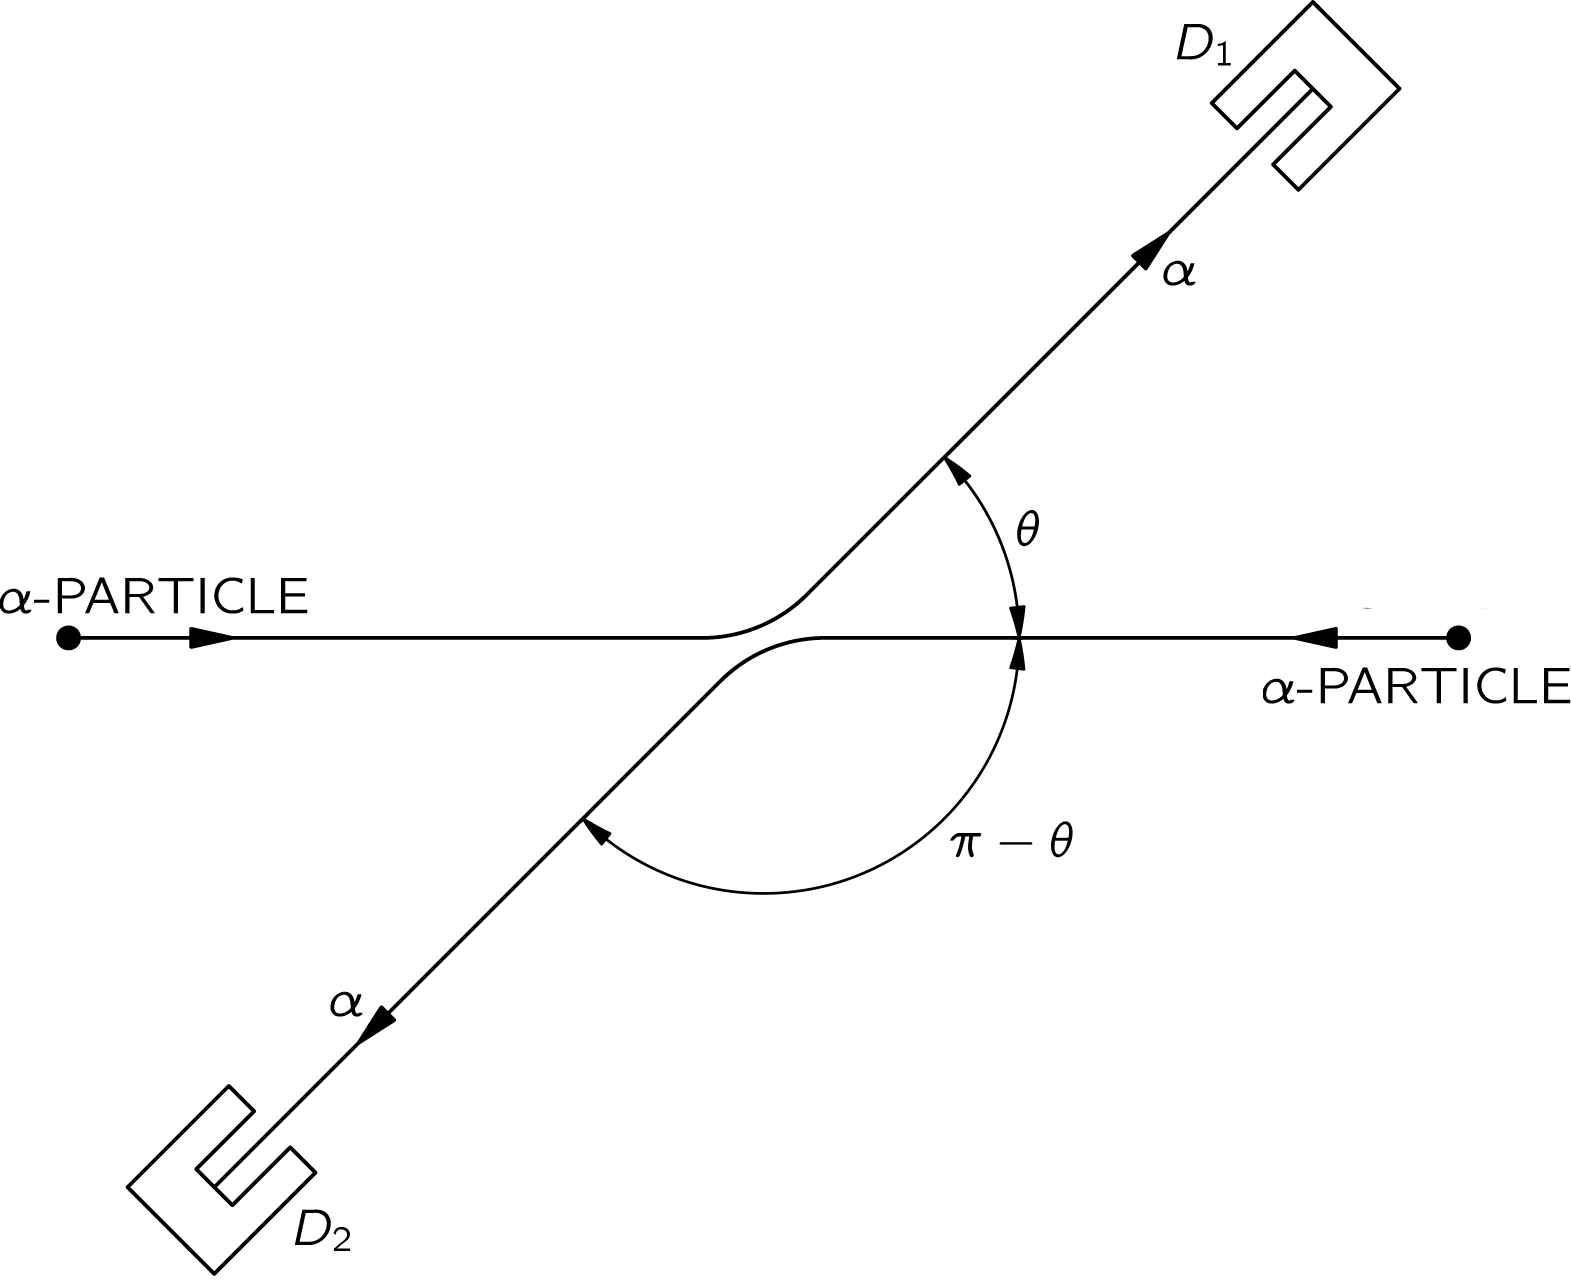
\includegraphics[scale=0.45]{alpha-alpha.png}

 
	\columnbreak
	
		\begin{itemize}

			\item Consider if both are $ \alpha $ particles, \pause \newline
			\item Then we would not know which particle entered the detector, so the total probability changes to,  \pause \newline
			\item  The probability of a $ \alpha $ particle 
		being detected at detector 1 = $ \rvert\,f(\theta) + f(\pi - \theta) \rvert\,^{2} $
		
		\end{itemize}
	
	\end{multicols}
 	
\end{frame}

\begin{frame}

	\begin{multicols}{2}
 
  		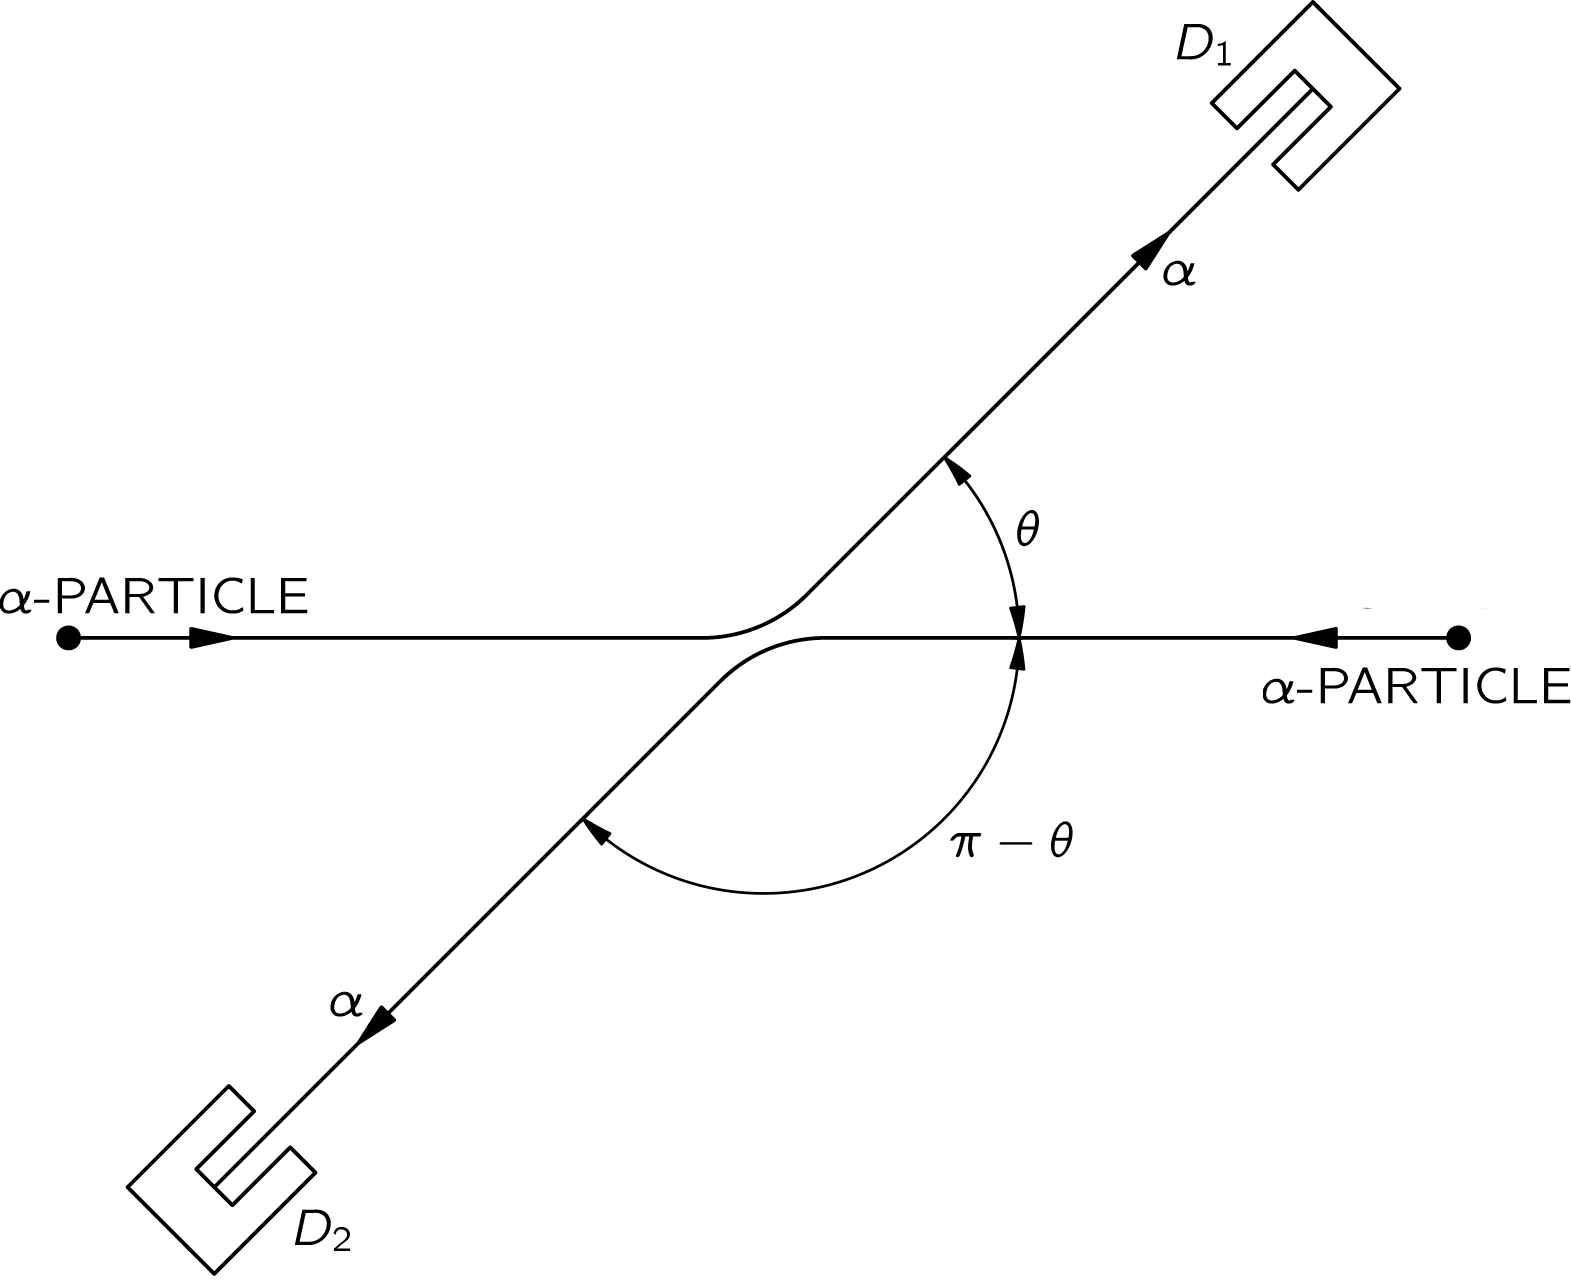
\includegraphics[scale=0.45]{alpha-alpha.png}
  
	\columnbreak
	
		\begin{itemize}

			\item If  $\theta = \dfrac{\pi}{2}$,  then applying this to the expression  $\rvert\,f(\theta)+f(\pi-\theta)\rvert\,^{2}$ we get, \pause \newline
			\item Probability = $4 \rvert\,f\left(\dfrac{\pi}{2}\right) \rvert\,^{2}$ , if the particles are indistinguishable.
		
		\end{itemize}
	
	\end{multicols}

	
\end{frame}

\begin{frame}{}

	\begin{multicols}{2}
 
   		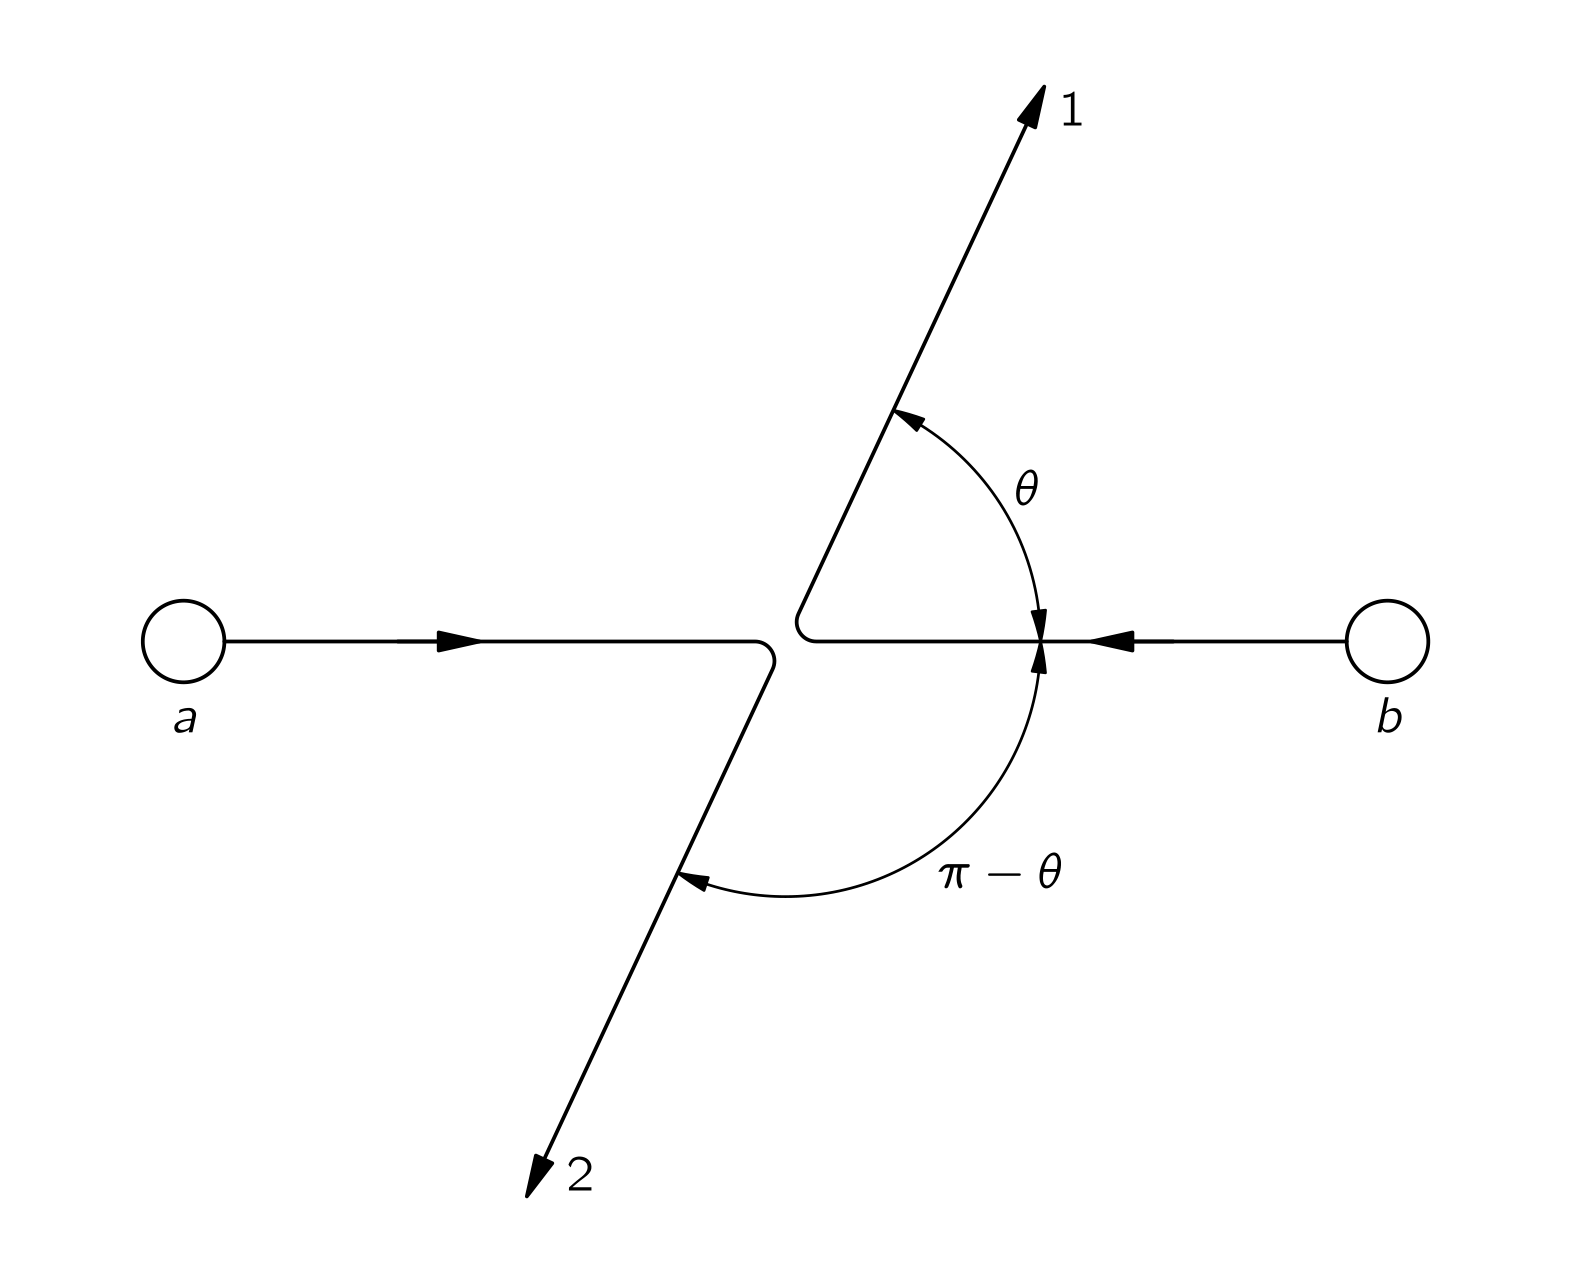
\includegraphics[scale=0.45]{a-b.png}

	\columnbreak
	
		\begin{itemize}

			\item Suppose the particles were distinguishable, then the probability for $\theta = \dfrac{\pi}{2}$ when applied for \[ \rvert\,f(\theta) \rvert\,^{2} + \rvert\,f(\pi - \theta) \rvert\,^{2} \] is given by \pause \newline
			\item Probability = $2 \Bigr\rvert\, f\left(\dfrac{\pi}{2}\right) \Bigr\rvert ^{2}$ \pause \newline 
			\item This shows that the probability gets doubled for indistinguishable particles.

		\end{itemize}
	
	\end{multicols}

	
\end{frame}

\begin{frame}
	
	\begin{itemize}
		\item \textit{Can we apply the same logic to the electron-electron scattering ? }\pause \newline
		\item \textit{OBSERVATION}: When we have situation in which the identity of the electron which is arriving at a point is exchanged with another one, the new amplitude interfere with old one with an opposite phase. \pause \newline
		\item In electrons case , the interfering amplitude for exchange interfere with a negative sign. \pause \newline
		Probability for electron = $\rvert\,f(\theta)-f(\pi-\theta)\rvert\,^{2}$
		 \end{itemize}
\end{frame}

\begin{frame}
\begin{tabular}{|c|cc|cc|c|}
\hline
Fraction of cases & Particle 1 & Particle 2 & Spin at D1 & Spin at D2 & Probability \\ \hline
$\frac{1}{4}$ & up & up & up & up & $\rvert\,f(\theta)-f(\pi-\theta)\rvert\,^{2}$ \\ \hline
$\frac{1}{4}$ & down & down & down & down & $\rvert\,f(\theta)-f(\pi-\theta)\rvert\,^{2}$ \\ \hline
$\frac{1}{4}$ & up & down & up & down & $\rvert\,f(\theta)\rvert\,^{2}$ \\ \cline{4-6}
 &  &  & down & up & $\rvert\,f(\pi -\theta)\rvert\,^{2}$ \\ \hline
$\frac{1}{4}$ & down & up & up & down & $\rvert\,f(\pi-\theta)\rvert\,^{2}$ \\ \cline{4-6}
& & & down & up & $\rvert\,f(\theta)\rvert\,^{2}$ \\ \hline
\end{tabular}
\end{frame}

\begin{frame}
	\frametitle{Identical Particles}
	
		{\large \textbf{Identical particles}\,, also called \textbf{indistinguishable particle}\,, are particles that cannot be distinguished from one another.}
		
\end{frame}

\begin{frame}{Identical indistinguishable particles}
	\begin{itemize}
		\item Consider particle 'a' and particle 'b'. \pause \newline
		\item Let the two particle collide and get scattered in two different directions say '1' and '2' over a surface element $ds_{1}$ and $ds_{2}$ of the detector respectively. \pause \newline
		\item If the particles are indistinguishable then the amplitudes of these process will add up. \pause \newline
		\item Probability that the two particles arrive at $ds_{1}$ and $ds_{2}$ is \pause \newline
		\[\rvert\braket{1|a}\braket{2|b} + \braket{2|a}\braket{1|b}\rvert\,^{2} ds_{1} ds_{2}\]
		
	\end{itemize}
\end{frame}

\begin{frame}
	\begin{itemize}
		\item Integrating over the area of the detector ,  if we let $ds_{1}$ and $ds_{2}$ range over the whole area $(\Delta S)$ , we could count each part of the area twice since the expression $\rvert\,\braket{1|a}\braket{2|b} + \braket{2|a}\braket{1|b}\rvert\,^{2} ds_{1} ds_{2}$ contains everything that can happen with any pair of surface elements $ds_{1}$ and $ds_{2}$. \pause \newline
		\item $ Probability_{BOSE} = \dfrac{ \left(4\,\rvert a \,\rvert^{2} \,\rvert b \,\rvert^{2}\right)}{2} \left(\Delta S\right)$ \pause \newline
		\item This is just twice what we got the probability for distinguished particles. 

	\end{itemize}
\end{frame}

\begin{frame}{State with n Bosons}
	\begin{itemize}
		\item Consider n particles say a, b, c\ldots scattered in n direction say 1, 2, 3 \ldots \pause \newline
		\item Probability that each particle acting alone would go into an element of the surface $ds$ of the detector is $\rvert \braket{ \cdots }\rvert^{2} ds$.
	\end{itemize}
\end{frame} 

\begin{frame}
	\begin{itemize}
		\item \textbf{Assumption}: All particles are distinguishable. \pause \newline
		\item Probability that n particles will be counted together in n different surface elements = $\rvert a_{1}b_{2}c_{3}\ldots \rvert^2ds_1ds_2\ldots$ \pause \newline
		\item If the amplitude does not depend on where ds is located in the detector , then the
		\[ Probability = \left(\rvert a \rvert^{2}\rvert b \rvert^{2}\ldots\right)(ds_{1}ds_{2}\ldots) \]
	\end{itemize}
\end{frame} 

\begin{frame}
	\begin{itemize}
		\item Integrating each dS over the surface $\Delta S$ of the dectector \pause \newline 
		$(P_{n})_{different} = \left(\rvert a \rvert^{2}\rvert b \rvert^{2}\ldots\right)(\Delta S)^{n}$ \pause \newline
		\item Now suppose that all the particle are bosons.
		\item For n particles, there are n! different , but indistinguishable  possibilities for which we must add the amplitudes. \pause \newline
	\end{itemize}
\end{frame}

\begin{frame}
	\begin{itemize}
	\item Probability that n particles will be counted on the n surface elements is given by \pause \newline $Probability = \left(\rvert a_{1}b_{2}c_{3}\ldots + a_{1}b_{3}c_{2}\ldots \rvert^{2}\right)(ds_{1}ds_{2}\ldots)$
	\item $Probability = \left(\rvert n!abc\ldots \rvert^{2}\right)(ds_{1}ds_{2}\ldots)$
	\item Integrate each ds over the area $\Delta S$ of the detector \pause \newline
	$(P_{n})_{BOSE} = n!\left(\rvert abc\ldots \rvert^{2}\right)(\Delta S)^{n}$
	\end{itemize}
\end{frame}

\begin{frame}
	\begin{itemize}
	\item Comparing the probability when the particles are distinguishable and indistinguishable \pause \newline
	$(P_{n})_{BOSE} = n!\left(\rvert abc\ldots \rvert^{2}\right)(\Delta S)^{n}$ \pause \newline
	$(P_{n})_{different} = \left(\rvert a \rvert^{2}\rvert b \rvert^{2}\ldots\right)(\Delta S)^{n}$ 
	\item $(P_{n})_{BOSE} = n!(P_{n})_{different}$
	\end{itemize}
\end{frame}

\begin{frame}
	\begin{itemize}
		\item What is the probability that a boson will go into particular state when there are already n particles present ?
	\end{itemize}
\end{frame}

\begin{frame}{Emission and Absorption of photons}
	\begin{itemize}
		\item When the light is emitted, a photon is "created".\pause \newline
		\item Consider that there are some atom emitting n photons. \pause \newline
		\item \textit{OBSERVATION}: The probability that an atom will emit a photon into a particular final state is increased by the factor (n+1) if there are already n photons in that state.
	\end{itemize}
\end{frame}

\begin{frame}
	\begin{itemize}
		\item In quantum mechanics we can show that \pause \newline 
		$\braket{\chi|\phi} = \braket{\phi|\chi}^{*}$ \pause \newline
		\item The amplitude to get from any condition $\phi$ to any other condition $\chi$. \pause \newline
		\item We have that amplitude that a photon will be added to some state, say j, when there are already n photons present we can express this condition as \pause \newline
		$\braket{n+1|n}=(\sqrt{n+1})a$\pause \newline
		$\braket{n|n+1}=\left(\sqrt{n+1}\right)a^{*}$ \pause \newline
		where $a = \braket{j|a}$ is the amplitude when there are no other photons are present.
	
	\end{itemize}
\end{frame}

\begin{frame}
	\begin{itemize}
		\item The amplitude to absorb a photon when there are n photons present is given by \pause \newline
		$\braket{n-1|n} = (\sqrt{n})a^{*}$ \pause \newline
		\item  $\braket{n+1|n}=(\sqrt{n+1})a$\pause \newline
		$\braket{n|n+1}=\left(\sqrt{n+1}\right)a^{*}$ \pause \newline
		\item The above two equation shows that they are symmetric in nature.
	\end{itemize}
\end{frame}

\begin{frame}
	\begin{itemize}
		\item \textit{Thought Experiment}: Lets us consider that there are n photons that are created in the same state, that of same frequency but they cannot be distinguished .\pause \newline
		\item The probability that an atom can emit another poton into same state is \pause \newline
		$(Probability)_{emit} = (n+1)\rvert\,a \rvert\,^{2}$  \pause \newline
		\item The probability that an atom absorbs a photon into the same state is \pause \newline
		$(Probability)_{absorb} = (n)\rvert\, a\rvert\,^{2}$
	\end{itemize}
\end{frame}

\begin{frame}
	\begin{itemize}
		\item Rate at which an atom will make a transition to downwards has two parts.\pause \newline
		\item Probability that it will make a spontaneous transition $\rvert a \rvert^{2}$  is proportional to the number of photons. \pause \newline
		\item The co-efficient of absorption, of induced emission and spontaneous emission are all equal and are related to the probability of spontaneous emission.
	\end{itemize}
\end{frame}

\begin{frame}{The Blackbody Spectrum}
	\begin{itemize}
	 \item For each light frequency $\omega$, there are certain N number of atoms which have two energy states separated, given by the equation $E = \omega\hbar$. \pause \newline
	 \item Let $N_e$ and $N_g$ be the average numbers of atoms that are in excited state and ground state. \pause \newline
	 \item In thermal equilibrium at temperature T, from statistical mechanics \pause \newline
	 $\frac{N_e}{N_g} = e^{\left(\dfrac{-\Delta E}{\omega\hbar}\right)}$  \pause \newline
	\item NOTE: Each atom in the ground state can absorb a photon and go into the excited state and each atom in the excited state can emit a photon and go to the ground state.
	\end{itemize}
\end{frame} 

\begin{frame}
	\begin{itemize}
		\item At equilibrium, the rate of these two process must be equal. \pause \newline
		\item Rate is proportional to the probability of the event and the number of atoms present.\pause \newline
		\item $\overline{n}$ is the average number of photons present in a given state with the frequency $\omega$.
	\end{itemize}
\end{frame}

\begin{frame}
	\begin{itemize}
		\item The absorption rate from the state is $N_{g}\overline{n}\rvert\,a\rvert\,^{2}$ , and the emission rate into that state is $N_{e}(\overline{n}+1)\rvert\,a\rvert\,^{2}$.
		\item At equilibrium  $N_{g}\overline{n}\rvert\,a\rvert\,^{2} = N_{e}(\overline{n}+1)\rvert\,a\rvert\,^{2}$
	\end{itemize}
\end{frame}

\begin{frame}
	\begin{itemize}
		\item Solving for the average number of photons present in a given state with the frequency $\omega$ \pause \newline
		$\overline{n} = \dfrac{1}{e^{\hbar\omega/k_{B}T} - 1}$ \pause \newline
		\item The energy of each photon is given by $\dfrac{\hbar\omega}{e^{\hbar\omega}/{k_{B}t} - 1}$ \pause \newline
		\item For any harmonic oscillator, the quantum mechanical energy levels are equally spaced with a seperation $\hbar\omega$.
	\end{itemize}
\end{frame}

\begin{frame}
	\begin{itemize}
		\item The energy levels are equally spaced and the $n^{th}$ energy level is the the mean enegry of the oscillator. \pause \newline 
		\center $(E)_{mean} = \dfrac{\hbar\omega}{e^{\hbar\omega/k_{B}t} - 1}$ \pause \newline
		\item Considering the boson which do not interact with each other, and in that state the whole system of particles behaves (for all quantum mechanical purpose) exactly like an harmonic oscillator. 
	\end{itemize}
\end{frame}

\begin{frame}
	\begin{itemize}
		\item Analysing the Electro-magnetic field in a box, it show the properties of an harmonic oscillation.
		\item Thus, the number of photons in a particular state in a box, can be equated to the number of energy levels associated with the particular modes of oscillation of the electromagnetic fields. 
	\end{itemize}
\end{frame}

\begin{frame}
	\begin{itemize}
		\item Mean energy in any particular modes in a box at a temperature T is given by  \pause \newline
		\center $(E)_{mean} = \dfrac{\hbar\omega}{e^{\hbar\omega/k_{B}t} - 1}$\pause \newline
	\end{itemize}
\end{frame} 


\begin{frame}
	\textit{ASSUMPTION}
	
		\begin{center}
		
		{\large For every mode there are some atoms in the box, which have energy levels that can radiate into that mode so that each mode can get into thermal equilibrium.}
	\end{center}
	
\end{frame}

\begin{frame}
	\begin{itemize}
		\item There will be billions of modes in the box and there will be many small frequency intervals $\Delta\omega$.
		
	\end{itemize}
	 \center 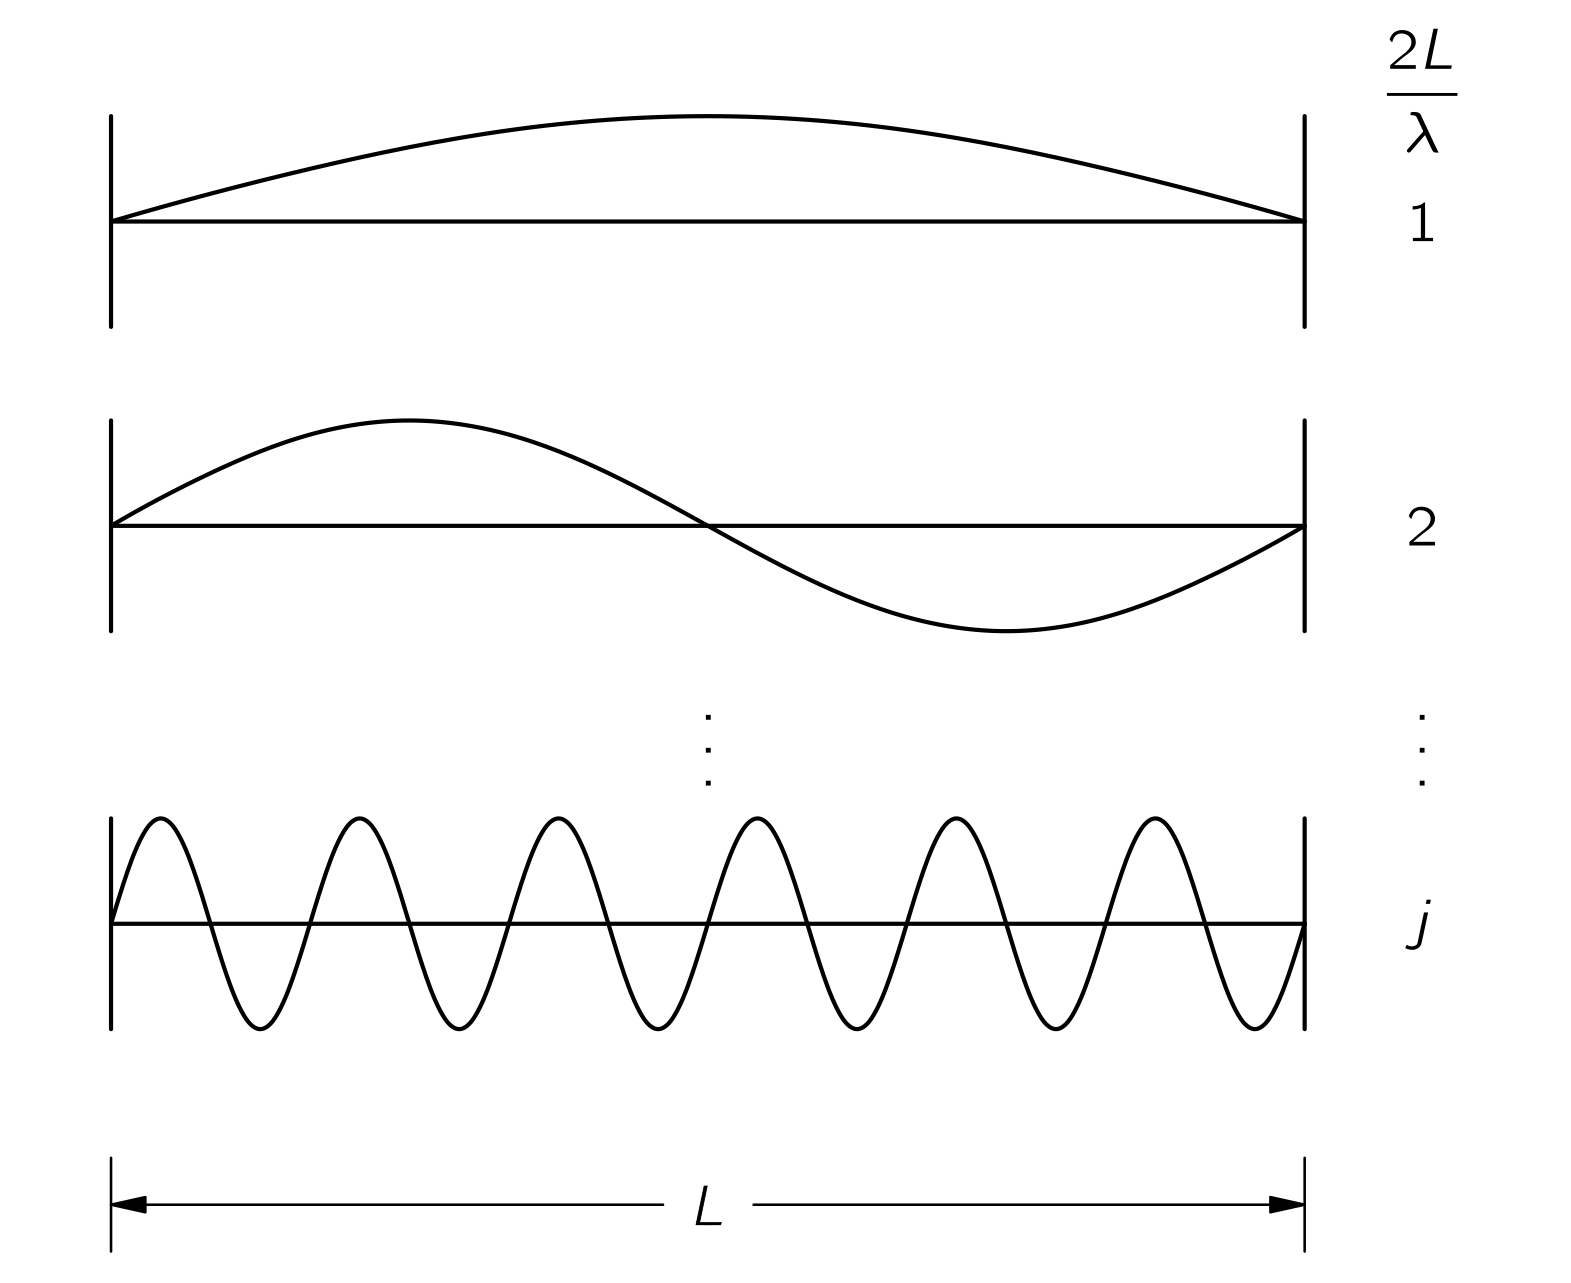
\includegraphics[scale=0.6]{modes.png}
\end{frame}

\begin{frame}
	\begin{itemize}
		\item The wave number k is given by $k = \dfrac{j\pi}{\lambda}$.
		\item The $\delta k$ between successive modes is given by \pause \newline
		
			$ \delta k = k_{j+1} - k_{j} = \dfrac{\pi}{L}$\pause \newline
			
		\item An assumption is made that kL is large that in small interval $\Delta k$, there are many modes. 	
		
		 
	\end{itemize}
\end{frame}

\begin{frame}
	\begin{itemize}
		\item $\Delta W$ is the number of modes in the interval $\Delta k$.\pause \newline
		\item This is given by $\Delta W = \dfrac{\Delta k}{\delta k}$ and $\delta k = \dfrac{j\pi}{L}$.\pause \newline
		\item Thus, $ \Delta W = \dfrac{L (\Delta k)}{\pi}$ \pause \newline 
		   \[ \boxed{\Delta W = \dfrac{L (\Delta k)}{2\pi}} \]
	\end{itemize}
\end{frame}

\begin{frame}
 \center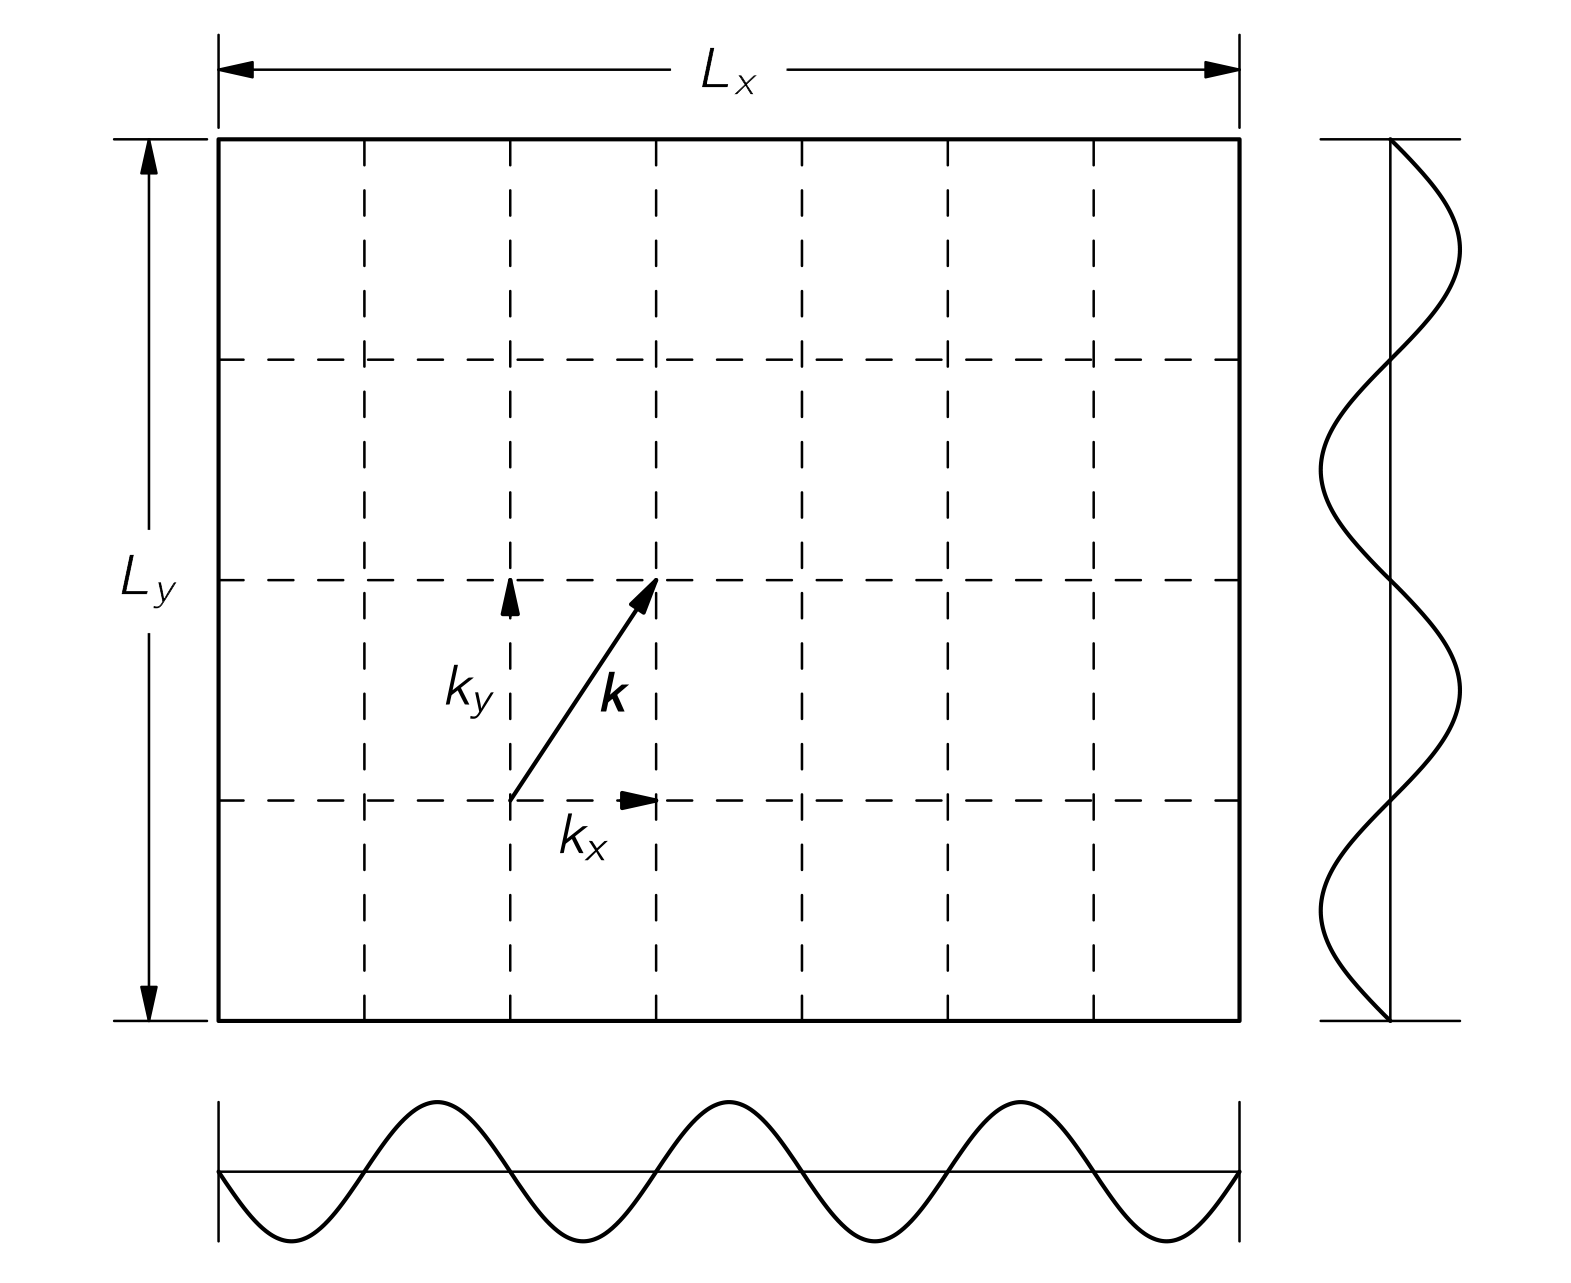
\includegraphics[scale=0.75]{k-space.png}
\end{frame}

\begin{frame}
	\begin{itemize}
		\item A standing wave in a rectangular box must have an integral number of half waves along each axis.
		\item Thus, $\Delta W$ the number of modes for a vector wave number \textbf{k} between the axes components $k$ and $k+\Delta k$ is \pause \newline
		
		\begin{align}
			\Delta W &= \dfrac{L_{x}L_{y}L_{z}}{(2\pi)^3}(\Delta k_{x}\Delta k_{y} \Delta k_{z}) \\[2ex]
			dW(K) &= V\dfrac{d^3k}{(2\pi)^3}
		\end{align}
		
	\end{itemize}
\end{frame}

\begin{frame}
	\begin{itemize}
		\item Applying the above result to find number of photon modes for photons with frequencies in the range $\Delta k$.
		\item In vacuum the magnitude of $\mathbf{k}$ is related to the frequency by \pause \newline
		
		$ \rvert\,k\rvert\, = \dfrac{\omega}{c}$.\pause \newline
		\item In the frequency interval $\Delta \omega$, these are all the modes which correspond to k's with magnitude between k and $k + \Delta k$, independent of the direction.
		\item The "volume in the k-space" between $k$ and $k + \Delta k $ is a spherical shell of volume \pause \newline
		$ 4\pi(k^2)\Delta k$.
	\end{itemize}
\end{frame}

\begin{frame}
	\begin{itemize}
		\item The number of modes is then , \pause \newline
		\center $\Delta W = \dfrac{V4\pi k^2\Delta k}{(2\pi)^3}$.
		\pause \newline
		\item substitute $k = \dfrac{\omega}{c}$\pause \newline
		
		$ \Delta W(\omega) = \dfrac{V4\pi \omega^2 \Delta \omega}{(2\pi c )^3}$
		
	\end{itemize}
\end{frame}

\begin{frame}
	\begin{itemize}
	\item These modes are independent, we must for double the number of modes.
	\item This is given by,\pause \newline
	
	$ \Delta W(\omega) = \dfrac{V(\omega^3)\Delta \omega}{\pi^2 c^3}$  (for light).
	\end{itemize}
\end{frame}

\begin{frame}
	\begin{itemize}
		\item We have shown that each mode has an average the energy \pause \newline 
		$ \overline{n}\hbar\omega = \dfrac{\hbar\omega}{e^{\hbar\omega/k_{B}T} - 1}$\pause \newline
		\item Multiplying This by the number of modes, we get the energy $\Delta E$ in the modes that lie in the interval $\Delta\omega$ :
		\[\Delta E = \left( \dfrac{\hbar\omega}{e^{\hbar\omega/k_{B}T} - 1} \right) \left(\dfrac{V\omega^3\Delta \omega}{\pi^2 c^3}\ \right) \]
		
	\end{itemize}
\end{frame}

\begin{frame}
	\begin{center}
		{\large The photons are the bosons, which have tendency to try to get to all into the same state.}
	\end{center}
\end{frame}


\subsection{Amplitude-based description of identical particles}

\subsection{n-Boson systems}

\subsection{Probability-based emission and absorption of blackbodies}

\begin{frame}

	\begin{center}
{\Large Thank you}
	\end{center}
	
\end{frame}

\end{document}

